\documentclass[aspectratio=169]{beamer}
\usetheme{metropolis}

\title{Introduction to Data Science -- Python Basics}
\subtitle{TA Teaching Slides}
\author{Fatima Fares -- Teaching Assistant}
\date{\today}

\begin{document}

% Title Page
\maketitle

% ---------------------------
\section{File Handling}
\begin{frame}[fragile]{File Handling Basics}
\begin{itemize}
  \item Open a file with: \texttt{open(filename, mode)}
  \item Modes: \texttt{'r'} (read), \texttt{'w'} (write), \texttt{'a'} (append)
  \item Example:
  \begin{verbatim}
  f = open('fout.txt', 'w')
  f.write("Hello World")
  f.close()
  \end{verbatim}
  \item Better practice:
  \begin{verbatim}
  with open('fout.txt', 'r') as f:
      content = f.read()
  \end{verbatim}
\end{itemize}
\end{frame}

% ---------------------------

\begin{frame}[fragile]{File Handling Quiz Example}
  \centering
  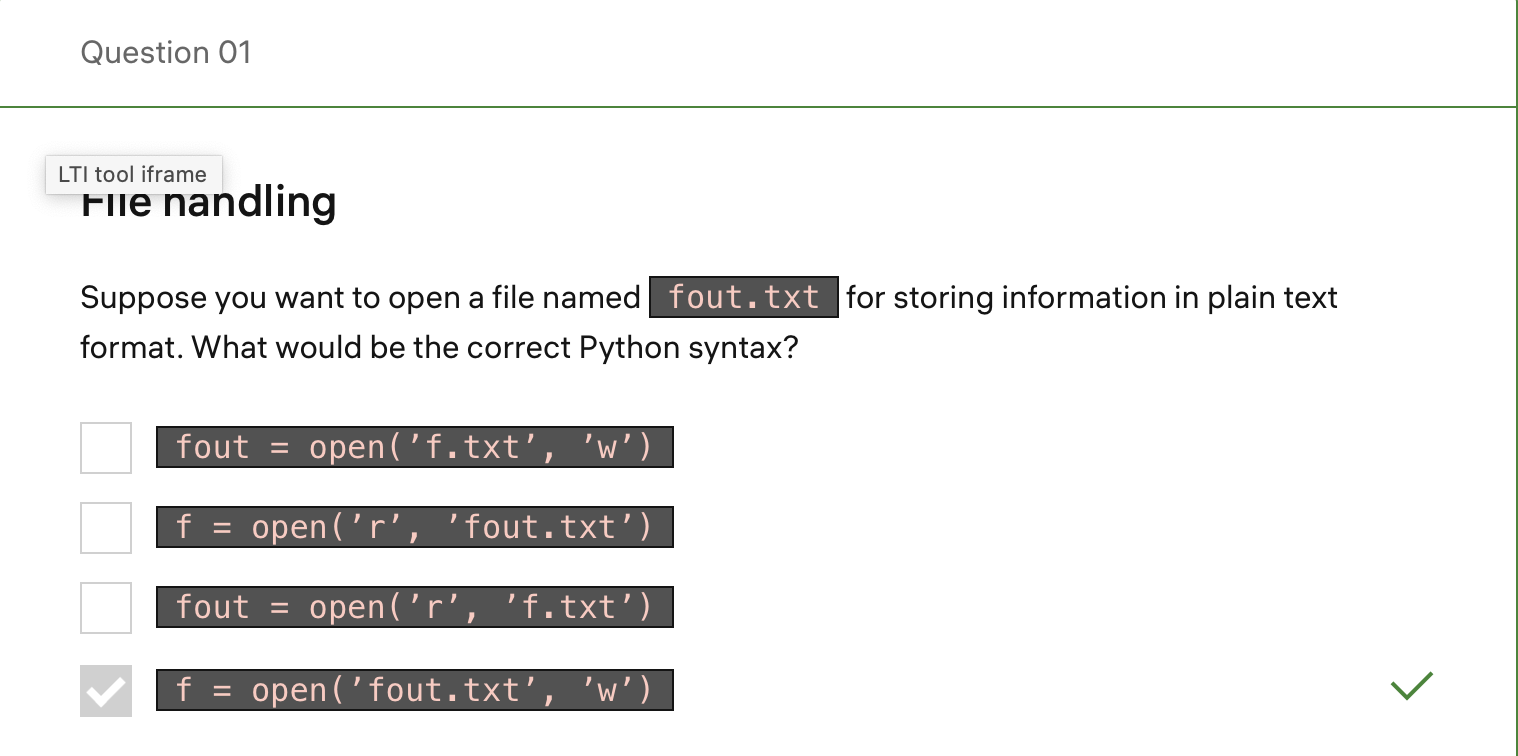
\includegraphics[width=0.9\textwidth]{screenshot.png}
\end{frame}


\section{Strings}
\end{frame}

\begin{frame}[fragile]{What is a String?}
\begin{itemize}
  \item A string is a sequence of characters stored as text.
  \item Strings are one of the most common Python data types.
  \item They are useful for storing names, words, and messages.
 \end{itemize}
\end{frame}

\begin{frame}[fragile]{Strings in Python}
\begin{itemize}
  \item Strings in Python are surrounded by either single or double quotation marks.
  \item Example: \texttt{'hello'} is the same as \texttt{"hello"}.
  \item You can display a string literal with the \texttt{print()} function.
\end{itemize}

\begin{verbatim}
print("hello")
print('hello')
\end{verbatim}

\end{frame}

\begin{frame}[fragile]{String Slicing Example}
\begin{verbatim}
s = 'abcdefgh'
print(s[3:-1:2])   
\end{verbatim}

\begin{itemize}
  \item String: \texttt{abcdefgh}
  \item Index positions: \texttt{a(0) b(1) c(2) d(3) e(4) f(5) g(6) h(7)}
  \item Slice format: \texttt{s[start:end:step]}
  \begin{itemize}
    \item start = 3 → begins at index 3 (\texttt{'d'})
    \item end = -1 → stops before the last char (\texttt{'h'})
    \item step = 2 → takes every 2nd character
  \end{itemize}
  \item Result: \texttt{'df'}
\end{itemize}
\end{frame}

\begin{frame}[fragile]{Tuples in Python}
\begin{itemize}
  \item Tuples are used to store multiple items in a single variable.
  \item One of 4 built-in collection data types in Python:
    \begin{itemize}
      \item List, Set, Dictionary, and Tuple
    \end{itemize}
  \item A Tuple is:
    \begin{itemize}
      \item \textbf{Ordered} (keeps the sequence of items)
      \item \textbf{Unchangeable} (immutable – cannot be modified)
    \end{itemize}
  \item Tuples are written with round brackets: \texttt{()}
\end{itemize}

\begin{verbatim}
# Example
tpl = ("apple", "banana", "cherry")
print(tpl[0])   # Output: apple
tpl[1] = "orange"   # ❌ Error: Tuples are immutable
\end{verbatim}
\end{frame}

\begin{frame}{Python Tuples Quiz Example}
  \centering
  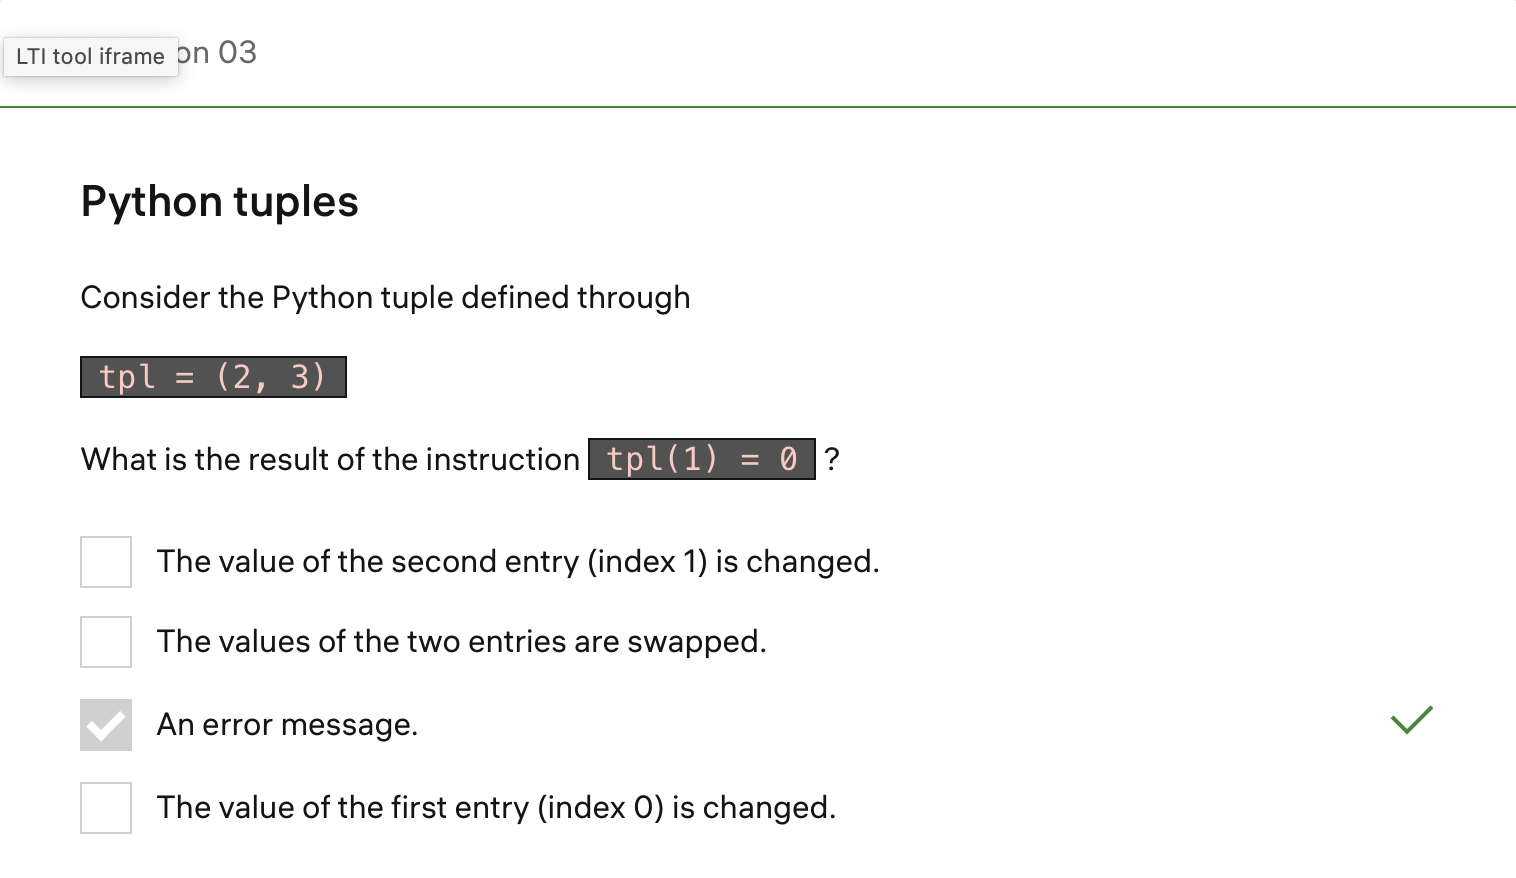
\includegraphics[width=0.9\textwidth]{tuples_quiz.png}
\end{frame}

\begin{frame}[fragile]{Python Lists}
\begin{itemize}
  \item Lists are used to store multiple items in a single variable.
  \item One of Python’s 4 built-in collection data types:
    \begin{itemize}
      \item List, Tuple, Set, Dictionary
    \end{itemize}
  \item A List is:
    \begin{itemize}
      \item \textbf{Ordered} – items have a defined order.
      \item \textbf{Changeable (mutable)} – items can be modified.
      \item \textbf{Allows duplicates}.
    \end{itemize}
  \item Lists are written with square brackets: \texttt{[]}
\end{itemize}

\begin{verbatim}
# Example
lst = ["apple", "banana", "cherry"]
print(lst[0])       # Output: apple

lst[1] = "orange"   # ✅ Allowed: lists are mutable
print(lst)          # ['apple', 'orange', 'cherry']
\end{verbatim}
\end{frame}

\begin{frame}{Python Lists Quiz Example}
  \centering
  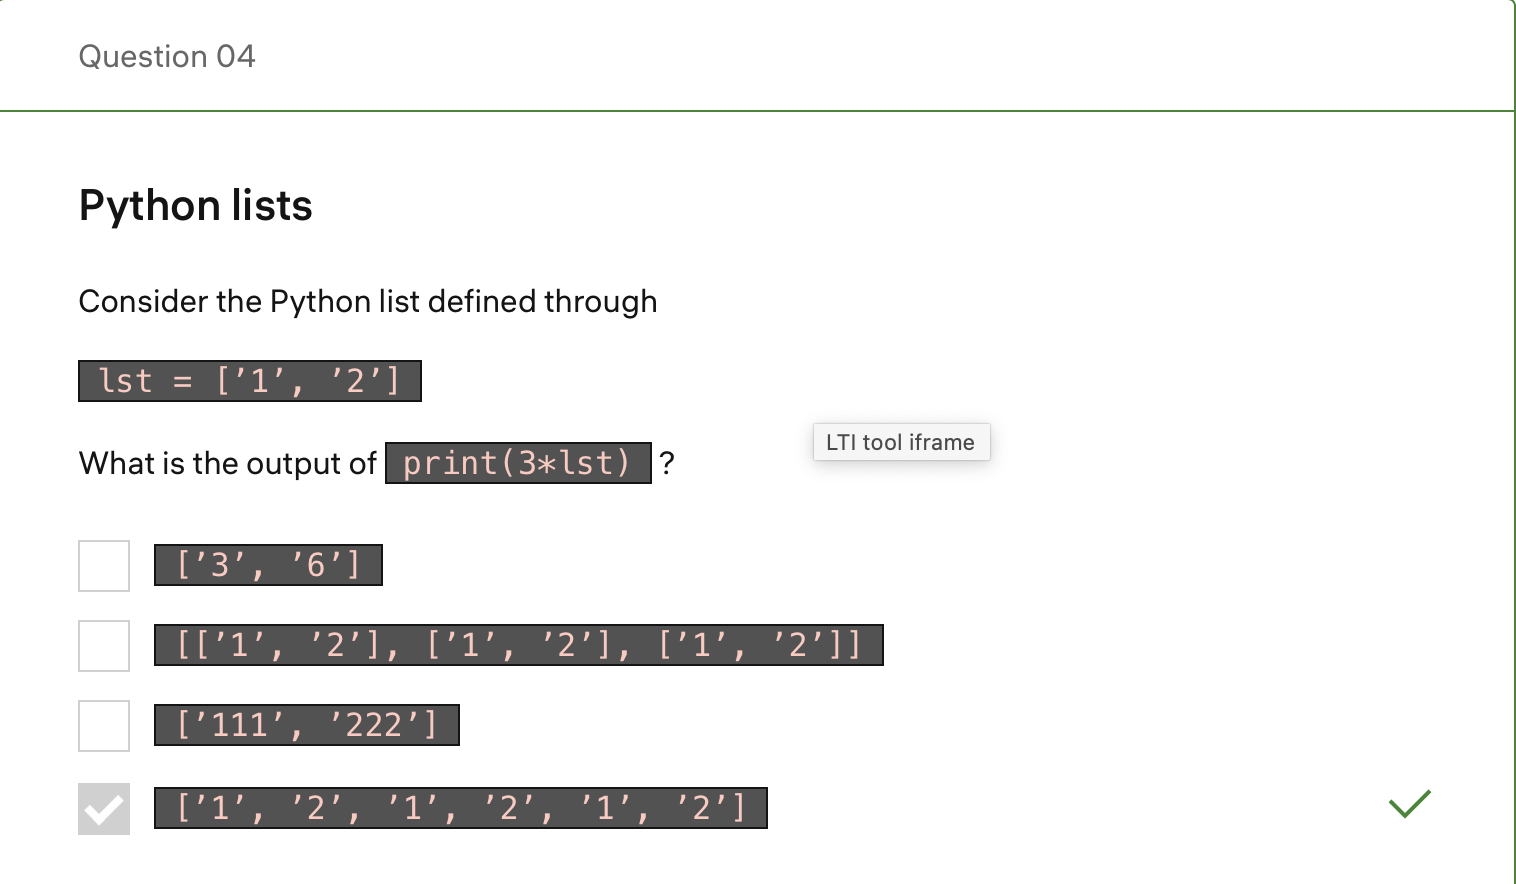
\includegraphics[width=0.9\textwidth]{lists_quiz.png}
\end{frame}


\end{document}